%=========================================================
% Security 
%=========================================================
\section{Security (Authentication)}
\label{sec:SECURITY}

The debug specification of RISC-V supports Security (Authentication). If security is enabled, only following accesses from JTAG/cJTAG are permitted.

\begin{enumerate}
    \item authenticated in dmstatus is readable.
    \item authbusy in dmstatus is readable.
    \item version in dmstatus is readable.
    \item dmactive in dmcontrol is readable and writable. 
    \item authdata is readable and writable.
\end{enumerate}

As shown in Figure \ref{fig:SECURITY}, there are three input signals related to security.\\
If DEBUG\_SECURE is Low, the security is disabled, so \seqsplit{DEBUG\_SECURE\_CODE\_0[31:0]} and \seqsplit{DEBUG\_SECURE\_CODE\_1[31:0]} are ignored.\\\\
If DEBUG\_SECURE is High, the security is enabled. The debug authentication is accepted if authdata matches to  \seqsplit{DEBUG\_SECURE\_CODE\_0[31:0]} or \seqsplit{DEBUG\_SECURE\_CODE\_1[31:0]}.\\\\
The reason why two secure codes are prepared is as follows. Usually the secure code is stored, for example, in non-volatile memory (FLASH, FUSE etc.) integrated in the chip by end-user. If the stored code is undefined in such case that the non-volatile memory has not been initialized due to the wafer being very fresh. In the case, if the secure is enabled and secure code is only one, it is impossible to match the authcode to the unknown code. So the mmRISC-1 receives two secure codes, and the one code is set by end-user, and the other code is fixed by chip manufacturer as secret master key. Even if the secure code defined by end-user is unknown, manufacturer can open the key.\\\\
When you want to set authdata from OpenOCD, write "riscv authdata\_write AUTHCODE" after "init" command in OpenOCD configuration file like as Listing \ref{list:SECURE_OPENOCD} which is based on USB-JTAG interface with FTDI FT2232D chip.


\begin{figure}[H]
    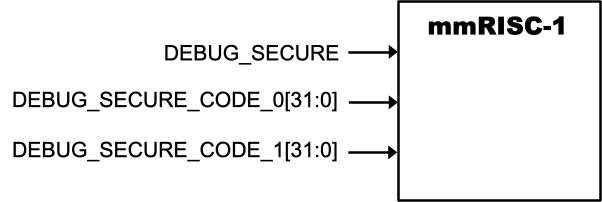
\includegraphics[width=0.75\columnwidth]{./Figure/Security.png}
    \caption{Security Configuration}
    \label{fig:SECURITY}
\end{figure}

\begin{lstlisting}[caption=Authentication Command in OpenOCD Configuration File, label=list:SECURE_OPENOCD, captionpos=b, frame=single, basicstyle=\ttfamily\scriptsize]
...
init
riscv authdata_write 0xbeefcafe
...
\end{lstlisting}




